\begin{filecontents*}{Grundlagen.rkt}
;; Die ersten drei Zeilen dieser Datei wurden von DrRacket eingefügt. Sie enthalten Metadaten
;; über die Sprachebene dieser Datei in einer Form, die DrRacket verarbeiten kann.
#reader(lib "DMdA-beginner-reader.ss" "deinprogramm")((modname Grundlagen) (read-case-sensitive #f) (teachpacks ()) (deinprogramm-settings #(#f write repeating-decimal #f #t none explicit #f ())))
; Achtung: Arithmetik mit Fliesskommazahlen (real)
unterliegt Rundung!
(+ 0.7
(- (/ 1/2 0.25)
(/ 0.6 0.3)))

(- (+ 0.7
(/ 1/2 0.25))
(/ 0.6 0.3))

; Arithmetik mit rationalen Zahlen (rational) ist exakt
(- (+ 7/10
(/ 1/2 1/4))
(/ 6/10 3/10))

(define absoluter-nullpunkt -273.15)
(define pi 3.141592653)
(define Gruendungsjahr-SC-Freiburg 1904)
(define top-level-domain-germany "de")
(define minutes-in-a-day (* 24 60))
(define vorwahl-tuebingen (sqrt 1/2))

; Abstraktion: Ausdruck mit "Loch" @$\odot$@
(lambda (@$\odot$@) (* @$\odot$@ (* 155 minutes-in-a-day)))


; Zuwachs der Weltbevoelkerung innerhalb von days Tagen
(define population-growth-in-days
(lambda (days) (* days (* 155 minutes-in-a-day))))

(population-growth-in-days 7)
\end{filecontents*}
\begin{filecontents*}{Uhr.rkt}
;; Die ersten drei Zeilen dieser Datei wurden von DrRacket eingefügt. Sie enthalten Metadaten
;; über die Sprachebene dieser Datei in einer Form, die DrRacket verarbeiten kann.
#reader(lib "DMdA-beginner-reader.ss" "deinprogramm")((modname Uhr) (read-case-sensitive #f) (teachpacks ()) (deinprogramm-settings #(#f write repeating-decimal #f #t none explicit #f ())))
; Grad, die Minutenzeiger pro Minute zuruecklegt
(define degrees-per-minute 360/60)

; Grad, die Stundenzeiger pro voller Stunde zuruecklegt
(define degrees-per-hour 360/12)

; Zeichne Ziffernblatt zur Stunde h und Minute m
(: draw-clock (natural natural -> image))
(check-expect (draw-clock 4 15) (draw-clock 16 15))
(define draw-clock
(lambda (h m)
(clock-face (position-hour-hand h m)
(position-minute-hand m))))

; Winkel (in Grad), den Minutenzeiger zur Minute m einnimmt
(: position-minute-hand (natural -> rational))
(check-expect (position-minute-hand 15) 90)
(check-expect (position-minute-hand 45) 270)
(define position-minute-hand
(lambda (m)
(* m degrees-per-minute)))

; Winkel (in Grad), den Stundenzeiger zur Stunde h einnimmt
(: position-hour-hand (natural natural -> rational))
(check-expect (position-hour-hand 3 0) 90)
(check-expect (position-hour-hand 18 30) 195)
(define position-hour-hand
(lambda (h m)
(+ (* (modulo h 12) degrees-per-hour)
; h mod 12 in {0,1,...,11}
(* (/ m 60) degrees-per-hour))))

; Zeichne Ziffernblatt mit Minutenzeiger um dm und
; Stundenzeiger um dh Grad gedreht
(: clock-face (rational rational -> image))
(define clock-face
(lambda (dh dm)
(clear-pinhole
(overlay/pinhole
(circle 50 "outline" "black")
(rotate (* -1 dh) (put-pinhole 0 35 (line 0 35 "red")))
(rotate (* -1 dm) (put-pinhole 0 45 (line 0 45 "blue")))))))

\end{filecontents*}
\begin{filecontents*}{myif.rkt}
; Bedingte Auswertung von e1 oder e2 (abhaengig von t1)
(check-expect (my-if (= 42 42) "Yes!" "No!") "Yes!")
(check-expect (my-if (odd? 42) "Yes!" "No!") "No!")
(define my-if
  (lambda (t1 e1 e2)
    (cond (t1 e1)
          (else e2))))

; Sichere Division x/y, auch fuer y = 0
(: safe-/ (real real -> real))
(define safe-/
  (lambda (x y)
    (my-if (= y 0)     ; <-- Funktion my-if wertet ihre Argumente
           x           ;     vor der Applikation aus: (/ x y) wird
           (/ x y))))  ;     in *jedem* Fall reduziert. :-(


(safe-/ 42 0)          ; Fuehrt zu Fehlemeldung "division by zero"
                       ; (Reduktion mit Stepper durchfuehren)
\end{filecontents*}
\begin{filecontents*}{Abs.rkt}
(: my-abs (real -> real))
(check-within (my-abs -4.2) 4.2 0.001)   ; Wichtig:
(check-within (my-abs 4.2) 4.2 0.001)    ; Tesfaelle decken alle Zweige
(check-within (my-abs 0) 0 0.001)        ; der conditional expression an
(define my-abs
  (lambda (x)
    (cond ((< x 0) (- x))
          ((> x 0) x    )
          (else    0    ))))
\end{filecontents*}
\begin{filecontents*}{andor.rkt}
(and #t #f)  ; @\eval@ #f   (Mathematik: Konjunktion)
(or #t #f)   ; @\eval@ #t   (Mathematik: Disjunktion)
; Kennzeichen am/pm fuer Stunde h
(: am/pm (natural -> (one-of "am" "pm" "???")))
(check-expect (am/pm 10) "am")
(check-expect (am/pm 13) "pm")
(check-expect (am/pm 25) "???")
(define am/pm
  (lambda (h)
    (cond ((and (>= h 0) (< h 12))  "am")
          ((and (>= h 12) (< h 24)) "pm")
          (else "???"))))
\end{filecontents*}
\begin{filecontents*}{records.rkt}
; Ein Charakter (character) besteht aus
; - Name (name)
; - Jedi-Status (jedi?)
; - Stärke der Macht (force)
(: make-character (string boolean real -> character))
(: character? (any -> boolean))
(: character-name (character -> string))
(: character-jedi? (character -> boolean))
(: character-force (character -> real))
(define-record-procedures character
  make-character
  character?
  (character-name
   character-jedi?
   character-force))


; Definiere verschiedene Charaktere des Star Wars Universums
(define luke
  (make-character "Luke Skywalker" #f 25))
(define r2d2
  (make-character "R2D2" #f 0))
(define dooku
  (make-character "Count Dooku" #f 80))
(define yoda
  (make-character "Yoda" #t 85))
\end{filecontents*}
\begin{filecontents*}{checkproperty.rkt}
(check-property 
 (for-all ((n string)
           (j boolean)
           (f real))
   (expect (character-name (make-character n j f)) n)))

(check-property 
 (for-all ((n string)
           (j boolean)
           (f real))
   (expect (character-jedi? (make-character n j f)) j)))

(check-property 
 (for-all ((n string)
           (j boolean)
           (f real))
   (expect-within (character-force (make-character n j f)) f 0.001)))
\end{filecontents*}
\begin{filecontents*}{forall.rkt}
; Für alle natürlichen Zahlen x1,x2 gilt: x1 + x2 @$\textcolor{kommentar}{\geq}$@ max(x1,x2)
(check-property
 (for-all ((x1 natural)
           (x2 natural))
   (>= (+ x1 x2) (max x1 x2))))
\end{filecontents*}
\begin{filecontents*}{konstruktor.rkt}
; Könnte Charakter c ein Sith sein?
(: sith? (character -> boolean))
(check-expect (sith? yoda) #f)
(check-expect (sith? r2d2) #f)
(define sith?
  (lambda (c)
    (and (not (character-jedi? c))
         (> (character-force c) 0))))


; Bilde den Charakter c zum Jedi aus (sofern c überhaupt Macht besitzt)
(: train-jedi (character -> character))

(check-expect (train-jedi luke) (make-character "Luke Skywalker" #t 50))
(check-expect (train-jedi r2d2) r2d2)

(define train-jedi
  (lambda (c)
    (make-character (character-name c) 
                    (> (character-force c) 0)
                    (* 2 (character-force c)))))
\end{filecontents*}
\begin{filecontents*}{latandlong.rkt}
; Ist x ein gültiger Breitengrad 
; zwischen Südpol (-90@\latexcode{$^{\circ}$}@) und Nordpol (90@\latexcode{$^{\circ}$}@)?
(: latitude? (real -> boolean))
(check-expect (latitude? 78) #t)
(check-expect (latitude? -92) #f)
(define latitude?
  (lambda (x)
    (within? -90 x 90)))
; Ist x ein gültiger Längengrad westlich (bis -180@\latexcode{$^{\circ}$}@) 
; bzw. östlich (bis 180@\latexcode{$^{\circ}$}@) des Meridians?
(: longitude? (real -> boolean))
(check-expect (longitude? 0) #t)
(check-expect (longitude? 200) #f)
(define longitude?
  (lambda (x)
    (within? -180 x 180)))
; Signaturen für Breiten-/Längengrade basierend auf
; den obigen Prädikaten
(define latitude
  (signature (predicate latitude?)))
(define longitude
  (signature (predicate longitude?)))
\end{filecontents*}
\begin{filecontents*}{oneoftopredicate.rkt}
(: f ((one-of 0 1 2 ) -> natural))
(define f
  (lambda (x)
    x))
; And then the "The Great one-of Extinction" of 2015 occurred @
\includegraphics[scale=0.5]{kaboon}@
(: g ((predicate 
       (lambda (x) (or (= x 0) (= x 1) (= x 2)))) -> natural))
(define g
  (lambda (x)
    x))
\end{filecontents*}
\begin{filecontents*}{geocoding.rkt}
(define geocoder-response
  (signature (mixed geocode geocode-error)))

(: sand13 geocoder-response)
(define sand13
  (geocoder "Sand 13, Tübingen"))

(geocode-address sand13)
(geocode-type sand13)
(location-lat (geocode-loc sand13))
(location-lng (geocode-loc sand13))
(geocode-accuracy sand13)
  

(: lady-liberty geocoder-response)
(define lady-liberty
  (geocoder "Statue of Liberty"))

(: alb geocoder-response)
(define alb
  (geocoder "Schwäbische Alb"))

(: A81 geocoder-response)
(define A81
  (geocoder "A81, Germany"))
\end{filecontents*}
\begin{filecontents*}{hemisphere.rkt}
; (Breitengrad < 0@\latexcode{$^{\circ}$}@?)
(: southern-hemisphere? (string -> boolean))

(check-expect (southern-hemisphere? "Cape Town") #t)
(check-expect (southern-hemisphere? "Tübingen") #f)
(check-error  (southern-hemisphere? "Mos Eisley") "Unknown location")

(define southern-hemisphere?
  (lambda (r)
    (let ((gc (geocoder r)))
      (cond ((geocode? gc)  
             (< (location-lat (geocode-loc gc)) 0))
            ((geocode-error? gc) 
             (violation "Unknown location"))))))
\end{filecontents*}
\begin{filecontents*}{distance.rkt}
;Abstand zweier geographischer Positionen l1, l2 auf der Erdkugel in km (lat, lng jeweils in Radian):
;dist(l1,l2) =
;   Erdradius in km *
;   acos(cos(l1.lat) * cos(l1.lng) * cos(l2.lat) * cos(l2.lng) + 
;        cos(l1.lat) * sin(l1.lng) * cos(l2.lat) * sin(l2.lng) +
;        sin(l1.lat) * sin(l2.lat))
; @\latexcode{$\pi$}@
(define pi 3.141592653589793)

; Konvertiere Grad d in Radian (@\latexcode{$\pi$}@ = @\latexcode{$180^{\circ}$}@)
(: radians (real -> real))
(check-within (radians 180) pi 0.001)
(check-within (radians -90) (* -1/2 pi) 0.001)
(define radians
  (lambda (d)
    (* d (/ pi 180))))


; Abstand zweier Orte o1, o2 auf Erdkugel (in km)
; [Wrapper]
(: distance (string string -> real))
(check-within (distance "Tübingen" "Freiburg") (distance "Freiburg" "Tübingen") 0.001)
(define distance
  (lambda (o1 o2)
    (let ((dist (lambda (l1 l2)             ; Abstand zweier Positionen l1, l2 (in km)  [Worker]
                  (let ((earth-radius 6378) ; Erdradius (in km)                  
                        (lat1 (radians (location-lat l1)))
                        (lng1 (radians (location-lng l1)))
                        (lat2 (radians (location-lat l2)))
                        (lng2 (radians (location-lng l2))))
                    (* earth-radius
                       (acos (+ (* (cos lat1) (cos lng1) (cos lat2) (cos lng2))
                                (* (cos lat1) (sin lng1) (cos lat2) (sin lng2))
                                (* (sin lat1) (sin lat2))))))))
          (gc1 (geocoder o1))
          (gc2 (geocoder o2)))
      (if (and (geocode? gc1)
               (geocode? gc2))
          (dist (geocode-loc gc1) (geocode-loc gc2))
          (violation "Unknown location(s)")))))

; ... einmal quer durch die schöne Republik
(distance "Konstanz" "Rostock")
\end{filecontents*}
\begin{filecontents*}{makepair.rkt}
; Ein paar aus natürlichen Zahlen
; FIFA WM 2014
(: deutschland-vs-brasilien (pair-of natural natural))
(define deutschland-vs-brasilien
  (make-pair 7 1)) 

; Ein Paar aus einer reellen Zahl (Messwert) 
; und einer Zeichenkette (Einheit)
(: measurement (pair-of real string))
(define measurement
  (make-pair 36.9 "@$^{\textcolor{string}{\circ}}$@C"))


; "Liste" der Zahlen 1,2,3,4
(define nested
  (make-pair 1
             (make-pair 2
                        (make-pair 3
                                   4))))

; Extrahiere das dritte Element der Liste (hier: 3)
(first (rest (rest nested)))
\end{filecontents*}
\begin{filecontents*}{lists.rkt}
; Noch einmal (jetzt mit Signatur): Liste der natürlichen Zahlen 1,2,3,4
(: one-to-four (list-of natural))
(define one-to-four
  (make-pair 1
             (make-pair 2
                        (make-pair 3
                                   (make-pair 4
                                              empty)))))


; Eine Liste, deren Elemente natürliche Zahlen oder Strings sind
(: abstiegskampf (list-of (mixed number string)))
(define abstiegskampf
  (make-pair "SCF"
             (make-pair 96
                        (make-pair "SCP"
                                   (make-pair "VfB" empty)))))


\end{filecontents*}
\begin{filecontents*}{nestedlist.rkt}
; Geschachtelte Listen
(: jedis-and-siths (list-of (list-of string)))
(define jedis-and-siths
  (MAKE-PAIR (make-pair "Yoda"
                        (make-pair "Obi-Wan" empty))
             (MAKE-PAIR (make-pair "Dooku"
                                   (make-pair "Vader" empty))
                        empty)))

; Navigation in geschachtelten Listen
(check-expect (first (first jedis-and-siths)) "Yoda")
(check-expect (first (rest (first (rest jedis-and-siths)))) "Vader")
\end{filecontents*}
\begin{filecontents*}{recursivelistlength.rkt}
; Länge der Liste xs
(: list-length ((list-of %a) -> natural))

(check-expect (list-length empty) 0)
(check-expect (list-length (list 1 1 3 8)) 4)
(check-expect (list-length jedis-and-siths) 2)    ; nicht 4!

(define list-length
  (lambda (xs)
    (cond ((empty? xs) 0)
          ((pair? xs) (+ 1 
                         (list-length (rest xs)))))))
\end{filecontents*}
\begin{filecontents*}{cat.rkt}
; Füge Listen xs, ys (in dieser Reihenfolge) zusammen
(: cat ((list-of %a) (list-of %a) -> (list-of %a)))

(check-expect (cat (list 1 2) (list 3 4)) (list 1 2 3 4))
(check-expect (cat one-to-four empty) one-to-four)
(check-expect (cat empty one-to-four) one-to-four)

(define cat
  (lambda (xs ys)
    (cond ((empty? xs) 
           ys)
            ((pair? xs)
             (make-pair (first xs) ; <- cat dennoch param. polymorph
                        (cat (rest xs) ys))))))

; Hinweis: Verfügbar als eingebaute Funktion `append'
\end{filecontents*}
\begin{filecontents*}{bluescreen.rkt}
(define yoda @
\includegraphics[scale=0.5]{Yoda}@)
(define dagobah @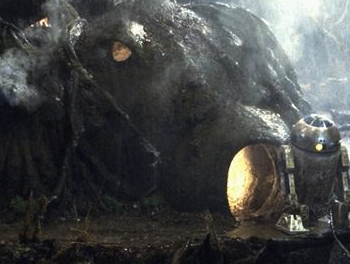
\includegraphics[scale =0.5]{dagobah}@)
;_________________________________________
;Zugriff auf die Liste der Bildpunkte (Pixel) eines Bildes: 
 
;(: image->color-list (image -> (list-of rgb-color)))  
;(: color-list->bitmap ((list-of rgb-color) natural natural -> image))
 
;Breite/Höhe eines Bildes in Pixeln:
 
;(: image-width (image -> natural))
; (: image-height (image -> natural))
 
; Eine Farbe (rgb-color) besteht aus ihrem
; - Rot-Anteil 0..255 (red)
; - Grün-Anteil 0..255 (green)
; - Blau-Anteil 0..255 (blue)

 @
\includegraphics[scale=0.5]{pixel}@
 
; (define-record-procedures rgb-color
;   make-color
;   color?
;   (color-red color-green color-blue))
;________________________________________

; Signatur für color-Records nicht in image2.rkt eingebaut.  Roll our own...
(define rgb-color
  (signature (predicate color?)))


; Ist Farbe c bläulich?
(: bluish? (rgb-color -> boolean))
(define bluish?
  (lambda (c)
    (< (/ (+ (color-red c) (color-green c) (color-blue c))
          3)
       (color-blue c))))

; Worker:
; Pixel aus Hintergrund bg scheint durch, wenn der
; entsprechende Pixel im Vordergrund fg bläulich ist.
; Arbeite die Pixellisten von fg und bg synchron ab
; Annahme: fg und bg haben identische Länge!
(: bluescreen ((list-of rgb-color) (list-of rgb-color) -> (list-of rgb-color)))
(define bluescreen
  (lambda (fg bg)
    (cond ((empty? fg)
           empty)
          ((pair? fg)
           (make-pair 
            (if (bluish? (first fg))
                (first bg)
                (first fg))
            (bluescreen (rest fg) (rest bg)))))))

; Wrapper:
; Mische Vordergrund fg und Hintergrund bg nach Bluescreen-Verfahren
(: mix (image image -> image))
(define mix
  (lambda (fg bg)
    (let ((fg-h (image-height fg))
          (fg-w (image-width fg))
          (bg-h (image-height bg))
          (bg-w (image-width bg)))
      (if (and (= fg-h bg-h)
               (= fg-w bg-w))
          (color-list->bitmap
           (bluescreen (image->color-list fg)
                       (image->color-list bg))
           fg-w
           fg-h)
          (violation "Dimensionen von Vorder-/Hintergrund verschieden")))))

; Yoda vor seine Hüte auf Dagobah setzen
(mix yoda dagobah) @\eval \ 
\includegraphics[scale=0.5]{Yoda_finished}@
\end{filecontents*}
\begin{filecontents*}{notquiteall.rkt}
; Eigenschaft nur auswerten, wenn n > 0 (==>)
(check-property
 (for-all ((n natural))
   (==> (> n 0)   
        (= (succ (pred n)) n))))
\end{filecontents*}
\begin{filecontents*}{Fakultaet.rkt}
; Berechne n!
(: factorial (natural -> natural))
(check-expect (factorial 0) 1)
(check-expect (factorial 3) 6)
(check-expect (factorial 10) 3628800)

(define factorial
  (lambda (n)
    (cond ((= n 0) 1)
          ((> n 0) (* n (factorial (- n 1)))))))
\end{filecontents*}
\begin{filecontents*}{FehlerRekursiv.rkt}
; Fehlerhaft: kein Fortschritt im rekursiven Aufruf
; => potentiell "unendliche" Reduktion
(define unfactorial
  (lambda (n)
    (cond ((= n 0) 1)
          ((> n 0) (* n (unfactorial n))))))

; Fehlerhaft: kein definierter Abbruch der Rekursion
; => Abbruch der Reduktion bei n = 0 ("cond: alle Tests ergaben #f")
(define not-factorial
  (lambda (n)
    (cond ((> n 0) (* n (not-factorial (- n 1)))))))
\end{filecontents*}
\begin{filecontents*}{Endrekursion.rkt}
;; Die ersten drei Zeilen dieser Datei wurden von DrRacket eingefügt. Sie enthalten Metadaten
;; über die Sprachebene dieser Datei in einer Form, die DrRacket verarbeiten kann.
#reader(lib "DMdA-vanilla-reader.ss" "deinprogramm")((modname definitions) (read-case-sensitive #f) (teachpacks ((lib "image2.ss" "teachpack" "deinprogramm"))) (deinprogramm-settings #(#f write repeating-decimal #f #t none explicit #f ((lib "image2.ss" "teachpack" "deinprogramm")))))
; Messung der Reduktionszeit (in Millisekunden) 
; für Ausdruck <e> mittels (time <e>)
(require racket/base)  


; Erinnerung: Generiere Liste von s bis e
(: from-to (natural natural -> (list-of natural)))
(define from-to
  (lambda (s e)
    (cond ((> s e) empty)
          (else (make-pair s (from-to (+ s 1) e)))))) 


; Erinnerung: konkateniere Listen xs und ys
; (Länge von xs bestimmt Anzahl rekursiver Aufrufe)

(: cat ((list-of %a) (list-of %a) -> (list-of %a)))  
(define cat
  (lambda (xs ys)
    (cond ((empty? xs) 
           ys)
          ((pair? xs)
           (make-pair (first xs)
                      (cat (rest xs) ys))))))

; ------------------------------------------------------------------------------

; Berechne n! (nicht endrekursiv)
(: factorial (natural -> natural))
(define factorial
  (lambda (n)
    (cond ((= n 0) 1)
          ((> n 0) (* n (factorial (- n 1)))))))
;                  ^^^^^^^^^^^^^^^^^^^^^^^^
;        nicht-leerer Kontext (* n ▢ ) des rekursiven Aufrufes
           

(factorial 5)


; Berechne n!
; Wrapper
(: fac (natural -> natural))
(check-expect (fac 0) 1)
(check-expect (fac 3) 6)
(define fac
  (lambda (n)
    (fac-worker n 1)))

; Berechne n! (mit Zwischenergebnis/Akkumulator acc), endrekursiv
; Worker
(define fac-worker
  (lambda (n acc)
    (cond ((= n 0) acc)
          ((> n 0) (fac-worker (- n 1) (* n acc))))))
;                  ^^^^^^^^^^^^^^^^^^^^^^^^^^^^^^
;                  endrekursiver Aufruf (tail call)
;                  siehe Syntaxprüfung (rosa Pfeile)

(fac 5)



; Liste xs umdrehen
; Aufwand: 1/2 × n × (n + 1) Aufrufe von make-pair wenn xs die Länge n hat
(: rev ((list-of %a) -> (list-of %a)))

(check-expect (rev empty) empty)
(check-expect (rev (list 1 2 3 4)) (list 4 3 2 1))

(define rev
  (lambda (xs)
    (cond ((empty? xs) empty)
          ((pair? xs) 
           (cat (rev (rest xs)) (list (first xs)))))))


; Liste xs umdrehen (effiziente Variante)
; Wrapper
(: backwards ((list-of %a) -> (list-of %a)))

(check-expect (backwards empty) empty)
(check-expect (backwards (list 1 2 3 4)) (list 4 3 2 1))

(define backwards
  (lambda (xs)
    
    ; Liste xs umdrehen (mit Akkumulator acc, endrekursiv)
    ; Worker
    ; Aufwand: n Aufrufe von make-pair, wenn xs die Länge n hat
    (letrec ((backwards-worker
              (lambda (xs acc)
                (cond ((empty? xs) acc)
                      ((pair? xs) 
                       (backwards-worker (rest xs) (make-pair (first xs) acc)))))))
      
      (backwards-worker xs empty))))

; NB:
; Benutzt letrec, um die rekursive Worker-Definition lediglich
; lokal zu definieren.


; Performance-Test: Umdrehen einer Liste von n = 1000 Elementen
;
; (1) Führt 1/2 × n × (n + 1) = 500500 Aufrufe von make-pair durch:
(time (rev (from-to 1 1000)))

; (2) Führt n = 1000 Aufrufe von make-pair durch:
(time (backwards (from-to 1 1000)))


; NB:
; backwards ist als Funktion `reverse' in DrRacket verfügbar
\end{filecontents*}